% ============================================================================
% Week 12 -- LECTURE NOTE (student-facing, board format)
%
% Data-driven two-stage LAP, part 1: the canonical MILP with uncertain data in a
% single stage (objective, then right-hand side), two stages and SAA, then the
% two-stage LAP and a numerical example on week 6's map. Part 2 (week 13)
% evaluates the plan.
% Style of week06-note.tex. Self-contained.
% ============================================================================
\documentclass[10pt]{article}

\usepackage[a4paper, margin=1.5cm]{geometry}
\usepackage{amsmath, amssymb}
\usepackage[dvipsnames]{xcolor}
\usepackage{graphicx}
\usepackage{array}
\usepackage{tikz}
\usetikzlibrary{matrix}
\usepackage{needspace}
\usepackage[hidelinks]{hyperref}

\definecolor{ruleink}{RGB}{18, 68, 140}
\definecolor{demoink}{RGB}{140, 82, 20}
\definecolor{keyink}{RGB}{20, 90, 20}
\definecolor{watchink}{RGB}{86, 60, 140}
\definecolor{punchink}{RGB}{170, 30, 60}

\setlength{\parindent}{0pt}
\pagestyle{empty}
\frenchspacing

% tighter spacing around centered displays
\AtBeginDocument{%
  \abovedisplayskip=4pt plus 1pt
  \belowdisplayskip=4pt plus 1pt
  \abovedisplayshortskip=2pt
  \belowdisplayshortskip=2pt}

% ---- one section -----------------------------------------------------------
\newcommand{\beat}[2]{%   number, title
  \par\medskip\needspace{8\baselineskip}%   never strand a title at the page foot
  {\color{ruleink}\rule{\textwidth}{1pt}}\par\nobreak\vspace{2pt}
  {\large\bfseries #1.\; #2}\par\nobreak\vspace{3pt}}

% ---- board content ---------------------------------------------------------
\newenvironment{board}{%
  \par\vspace{2pt}
  \begingroup\leftskip=1.3em\relax}{%
  \par\endgroup\vspace{2pt}}

% ---- highlights ------------------------------------------------------------
\newcommand{\demo}[2]{\par{\leavevmode\color{demoink}\small\textbf{demo}\quad\texttt{#1} --- #2}\par}
\newcommand{\watch}[1]{\par{\color{watchink}\small\textbf{watch}\quad #1}\par}
\newcommand{\key}[1]{\par\vspace{1pt}{\color{keyink}\small\textbf{KEY}\quad\textbf{#1}}\par}
\newcommand{\takeaway}[1]{%
  \par\vspace{2pt}\noindent
  {\color{punchink}\rule{2pt}{10pt}}\;{\color{punchink}\small\textbf{takeaway}\quad\textbf{#1}}\par\vspace{2pt}}

\begin{document}

{\Large\bfseries Week 12 --- Data-Driven Two-Stage LAP 1}\\[2pt]
{\small OL7014 Integer Programming \quad\textbullet\quad Instructor: Prof.\ H.\ Park \quad\textbullet\quad Week of Nov 9, 2026}

% ---------------------------------------------------------------- 1
\beat{1}{Uncertain data --- decide now, see later}
\begin{board}
week 1: every number known. \quad today: some data is \textbf{random} --- call it $\tilde{\xi}$, \ $\tilde{\xi} \sim \mathbb{P}$; \quad a realization is written $\xi$
\vspace{4pt}

\noindent
\begin{minipage}[t]{0.36\linewidth}
\centering
\textbf{Deterministic program} (week 1)
\[
\begin{aligned}
  \min_x\quad & f(x) \\
  \text{s.t.}\quad & x \in X
\end{aligned}
\]
\end{minipage}%
\hfill%
\begin{minipage}[t]{0.61\linewidth}
\centering
\textbf{Stochastic program}
\[
\boxed{\;
\begin{aligned}
  \min_x\quad & \mathbb{E}_{\mathbb{P}}\bigl[\, f(x, \tilde{\xi}) \,\bigr] \\
  \text{s.t.}\quad & x \in X \\
                   & \mathbb{P}\bigl(\, g(x, \tilde{\xi}) \le 0 \,\bigr) \ \ge\ 1 - \varepsilon
\end{aligned}
\;}
\qquad \text{(SP)}
\]
\end{minipage}%
\end{board}

% ---------------------------------------------------------------- 2
\beat{2}{The chance constraint --- a MIP}
\begin{board}
\[
  \mathbb{P}\bigl(\, g(x, \tilde{\xi}) \le 0 \,\bigr) \ \ge\ 1 - \varepsilon
  \qquad\Longleftrightarrow\qquad
  \mathbb{P}\bigl(\, g(x, \tilde{\xi}) > 0 \,\bigr) \ \le\ \varepsilon
\]
take $\mathbb{P}$ = the data: \ $N$ equally likely scenarios $\xi^1, \dots, \xi^N$ \ $\Rightarrow$ \ the probability is a \textbf{count}:
\[
  \frac{1}{N} \sum_{n=1}^{N} \mathbb{I}\bigl[\, g(x, \xi^n) > 0 \,\bigr] \ \le\ \varepsilon
  \qquad \text{--- at most $\varepsilon N$ scenarios may fail}
\]
\textbf{one binary per scenario} \ (week 2's big-$M$, week 4's trick): \quad $z^n = 1 \iff$ scenario $n$ may violate
\[
  g(x, \xi^n) \ \le\ M z^n
  \qquad\quad z^n = 0 \ \Rightarrow \ g(x, \xi^n) \le 0; \qquad z^n = 1 \ \Rightarrow \ \text{row says nothing} \quad (M \ge \max g)
\]
\[
\begin{aligned}
  \text{the MIP:}\qquad \min_{x,\, z}\quad & f(x) \\
  \text{s.t.}\quad & x \in X \\
                   & g(x, \xi^n) \le M z^n && \forall n \in [N] \\
                   & \textstyle\sum_{n=1}^{N} z^n \le \varepsilon N, \qquad z^n \in \{0,1\} && \forall n \in [N]
\end{aligned}
\]
$N = 100$, $\varepsilon = 0.05$: \ at most $5$ scenarios fail --- \emph{and the solver chooses which $5$}
\end{board}

% ---------------------------------------------------------------- 3
\beat{3}{Why the mean --- every plan has a cost distribution}
\begin{board}
fix $x$ \ $\Rightarrow$ \ $f(x, \tilde{\xi})$ is a random number --- it has a \emph{distribution}
\begin{center}
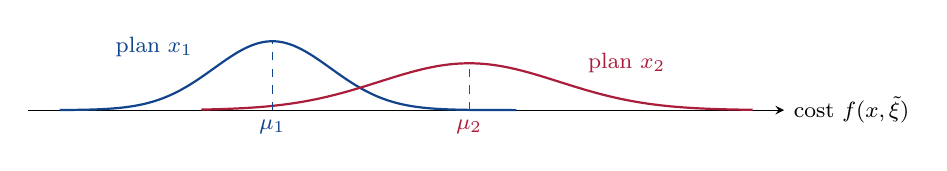
\begin{tikzpicture}[font=\footnotesize, >=stealth, yscale=0.7]
  \draw[->] (0,0) -- (9.6,0) node[right] {cost $f(x, \tilde{\xi})$};
  \draw[thick, ruleink, domain=0.4:6.2, smooth, samples=50] plot (\x, {1.25*exp(-(\x-3.1)*(\x-3.1)/1.1)});
  \draw[thick, punchink, domain=2.2:9.2, smooth, samples=50] plot (\x, {0.85*exp(-(\x-5.6)*(\x-5.6)/2.6)});
  \draw[dashed, ruleink] (3.1,0) -- (3.1,1.25);
  \draw[dashed, punchink] (5.6,0) -- (5.6,0.85);
  \node[ruleink] at (1.6,1.15) {plan $x_1$};
  \node[punchink] at (7.6,0.85) {plan $x_2$};
  \node[below, ruleink] at (3.1,0) {$\mu_1$};
  \node[below, punchink] at (5.6,0) {$\mu_2$};
\end{tikzpicture}
\end{center}
which plan is better? \ compare the means: \ $\mu_1 < \mu_2$ \ $\Rightarrow$ \ $x_1$. \qquad that is (SP): \ $\min_{x \in X} \mathbb{E}_{\mathbb{P}}[\, f(x, \tilde{\xi}) \,]$
\end{board}
\watch{the mean is one way to rank distributions. \ others: worst case, tail (CVaR). not today.}

% ---------------------------------------------------------------- 4
\beat{4}{SAA --- replace $\mathbb{P}$ by the data}
\begin{board}
$\mathbb{P}$ is unknown. \ what we have: \ $N$ past realizations of $\tilde{\xi}$: \ $\xi^1, \xi^2, \dots, \xi^N$ \ --- the \textbf{scenarios}
\vspace{3pt}

\textbf{Def.} \ \textbf{Sample Average Approximation (SAA)}:
\[
  \underbrace{\min_{x \in X}\ \ \mathbb{E}_{\mathbb{P}}\bigl[\, f(x, \tilde{\xi}) \,\bigr]}_{\text{true problem --- cannot compute}}
  \qquad\approx\qquad
  \underbrace{\min_{x \in X}\ \ \frac{1}{N} \sum_{n=1}^{N} f(x, \xi^n)}_{\text{SAA problem --- every number known again}}
\]
why: \ for a fixed $x$, \ $\frac{1}{N} \sum_{n} f(x, \xi^n) \to \mathbb{E}_{\mathbb{P}}[\, f(x, \tilde{\xi}) \,]$ \ as $N \to \infty$ \quad (law of large numbers)
\vspace{4pt}

\emph{classification:} \ $\xi^n = (\boldsymbol{x}_n, y_n)$, \ the $N$ labelled points
\[
  \min_{\theta}\ \ \frac{1}{N} \sum_{n=1}^{N} \mathbb{I}\bigl[\, y_n\,(\theta^{\top}\boldsymbol{x}_n) \le 0 \,\bigr]
  \qquad \text{--- week 4's model, exactly: \ week 4 \emph{was} SAA}
\]
``plug in the average'' here would mean one point $(\bar{\boldsymbol{x}}, \bar{y})$ --- meaningless
\end{board}
\takeaway{SAA is \emph{not} ``plug in the average'' --- it keeps every data point.}

% ---------------------------------------------------------------- 5
\newpage
\beat{5}{Two stages --- the cost is itself an optimization}
\begin{center}
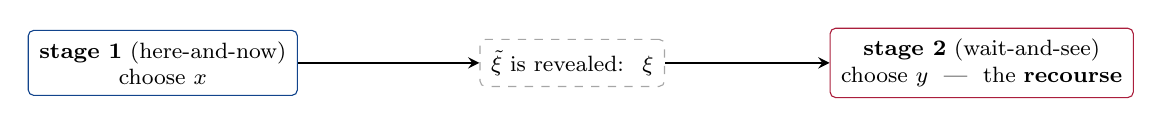
\begin{tikzpicture}[font=\footnotesize, >=stealth,
    st/.style={draw, rounded corners=2pt, inner sep=4pt, align=center}]
  \node[st, draw=ruleink] (s1) at (0,0) {\textbf{stage 1} (here-and-now)\\ choose $x$};
  \node[st, draw=gray!70, dashed] (ob) at (5.2,0) {$\tilde{\xi}$ is revealed: \ $\xi$};
  \node[st, draw=punchink] (s2) at (10.4,0) {\textbf{stage 2} (wait-and-see)\\ choose $y$ \ --- \ the \textbf{recourse}};
  \draw[->, thick] (s1) -- (ob);
  \draw[->, thick] (ob) -- (s2);
\end{tikzpicture}
\end{center}
\begin{board}
\begin{center}
\begin{tabular}{@{}l|l|l@{}}
 single stage & $f(x, \xi)$ = a formula & nothing left to decide after $\xi$ \\[3pt]
 \textbf{two stages} & $f(x, \xi) = c^{\top}x + Q(x, \xi)$ & after $\xi$ we still choose $y$ \\
\end{tabular}
\end{center}
stage 1: \ $x \in X$ --- week 2's MILP constraints, \ $X = \{\, x \in \mathbb{Z}^n_{+} : Ax \le b \,\}$. \qquad stage 2: new letters \ $q, \, T, \, W$
\vspace{3pt}

\textbf{Def.} \ the \textbf{recourse function} --- the best reaction, once $x$ is fixed and $\xi$ is seen:
\[
  Q(x, \xi) \;=\; \min_{y}\ \bigl\{\, q^{\top}y \ : \ Tx + Wy \ge \xi, \ \ y \ge 0 \,\bigr\}
  \qquad \text{$\xi$ = the right-hand side}
\]
(in general $\tilde{\xi}$ can be \emph{all} the stage-2 data $(q, T, W, h)$ --- today only the right-hand side is random)
\vspace{3pt}

same model, same SAA:
\[
  \min_{x \in X}\ \ c^{\top}x + \mathbb{E}_{\mathbb{P}}\bigl[\, Q(x, \tilde{\xi}) \,\bigr]
  \qquad\overset{\text{SAA}}{\Longrightarrow}\qquad
  \min_{x \in X}\ \ c^{\top}x + \frac{1}{N} \sum_{n=1}^{N} Q(x, \xi^n)
\]
write every $Q$ out --- one big MILP, the \textbf{extensive form}:
\[
  \min_{x,\ y^1, \dots, y^N}\ \ c^{\top}x + \frac{1}{N} \sum_{n=1}^{N} q^{\top}y^n
  \qquad \text{s.t.} \quad Tx + Wy^n \ge \xi^n \ \ (n = 1, \dots, N), \quad x \in X, \quad y^n \ge 0
\]
$N = 3$:
\[
  \begin{bmatrix} T & W &   &   \\ T &   & W &   \\ T &   &   & W \end{bmatrix}
  \begin{bmatrix} x \\ y^1 \\ y^2 \\ y^3 \end{bmatrix}
  \;\ge\;
  \begin{bmatrix} \xi^1 \\ \xi^2 \\ \xi^3 \end{bmatrix}
  \qquad\quad \text{one shared $x$; \ one block per scenario; \ plus $x \in X$}
\]
\end{board}
\takeaway{more data $\Rightarrow$ a bigger MILP: \ $N$ copies of $y$, \ $N$ copies of the rows.}

% ---------------------------------------------------------------- 6
\beat{6}{The two-stage LAP}
\begin{board}
week 6: \ $d = (12, 20, 8, 16, 24)$ was \emph{known} when we chose where to build. \ really?
\vspace{2pt}

the demand is random: \ $d \to \tilde{\xi}$, \quad $\xi^n_i$ = demand at node $i$ in scenario $n$
\begin{center}
\begin{tabular}{@{}l|l|l@{}}
 \textbf{stage 1} --- before the demand & $x_i$ \ open, \quad $r_i$ \ stock & no $n$ \\[3pt]
 \textbf{stage 2} --- after $\xi^n$ is seen & $y^n_{ij}$ \ ship, \quad $q^n_i$ \ unmet, \quad $s^n_i$ \ surplus & one copy per scenario \\
\end{tabular}
\end{center}
week 6's model, with $d \to \xi^n$ and a superscript $n$ on stage 2:
\[
  \min\quad
  \underbrace{\textstyle\sum_{i \in V} f_i x_i + \sum_{i \in V} h_i r_i}_{\text{stage 1}}
  \;+\; \frac{1}{N} \sum_{n=1}^{N}
  \underbrace{\Bigl[\, \textstyle\sum_{(i,j) \in E} c_{ij}\, y^n_{ij} + \sum_{i \in V} u_i\, q^n_i + \sum_{i \in V} o_i\, s^n_i \,\Bigr]}_{\text{stage 2, scenario $n$}}
\]
\vspace{-2pt}
\[
\begin{aligned}
  \text{s.t.}\quad
    & \textstyle\sum_{j} y^n_{ij} - \sum_{j} y^n_{ji} = r_i - \xi^n_i + q^n_i - s^n_i && (\forall i \in V, \ \forall n) && \text{[conservation, per scenario]} \\
    & \textstyle\sum_{i \in V} r_i \le B, \qquad r_i \le B\, x_i \ \ (\forall i \in V), \qquad \sum_{i \in V} x_i \le p && && \text{[stage 1: as in week 6]} \\
    & y^n, s^n \ge 0, \quad 0 \le q^n_i \le \xi^n_i, \quad r \ge 0, \quad x_i \in \{0,1\}
\end{aligned}
\]
$N = 1$: \ week 6's model, exactly
\vspace{2pt}

fix $(x, r)$ \ $\Rightarrow$ \ $N$ separate MCNFs (week 5) --- the hardness is still in $x$
\end{board}
\watch{$r$ is continuous but first-stage: \ the split is now by \emph{time}, not by integer vs.\ continuous.}

% ---------------------------------------------------------------- 7
\newpage
\beat{7}{Numerical example --- week 6's map, three futures}
\begin{center}
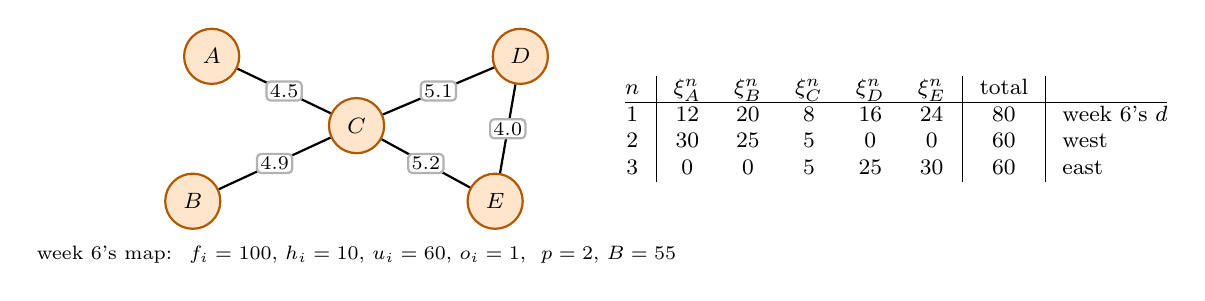
\begin{tikzpicture}[thick, font=\footnotesize, scale=0.8,
    site/.style={circle, draw=orange!70!black, fill=orange!20, minimum size=7mm},
    tt/.style={fill=white, draw=gray!60, rounded corners=1.5pt, inner sep=1.2pt, font=\scriptsize}]
  \node[site] (A) at (0, 1.6)    {$A$};
  \node[site] (B) at (-0.3, -0.7) {$B$};
  \node[site] (C) at (2.3, 0.5)   {$C$};
  \node[site] (D) at (4.9, 1.6)   {$D$};
  \node[site] (E) at (4.5, -0.7)  {$E$};
  \draw (A) -- node[tt] {$4.5$} (C);
  \draw (B) -- node[tt] {$4.9$} (C);
  \draw (C) -- node[tt] {$5.1$} (D);
  \draw (C) -- node[tt] {$5.2$} (E);
  \draw (D) -- node[tt] {$4.0$} (E);
  \node[font=\scriptsize] at (2.3, -1.55) {week 6's map: \ $f_i = 100$, $h_i = 10$, $u_i = 60$, $o_i = 1$, \ $p = 2$, $B = 55$};
  \node[anchor=west] at (6.4, 0.45) {%
    \begin{tabular}{@{}c|ccccc|c|l@{}}
      $n$ & $\xi^n_A$ & $\xi^n_B$ & $\xi^n_C$ & $\xi^n_D$ & $\xi^n_E$ & total & \\ \hline
      1 & 12 & 20 & 8 & 16 & 24 & 80 & week 6's $d$ \\
      2 & 30 & 25 & 5 & 0  & 0  & 60 & west \\
      3 & 0  & 0  & 5 & 25 & 30 & 60 & east \\
    \end{tabular}};
\end{tikzpicture}
\end{center}
\begin{board}
$N = 3$:
\[
  \min\quad 100 \textstyle\sum_i x_i + 10 \sum_i r_i
  \;+\; \displaystyle\frac{1}{3} \sum_{n=1}^{3}
  \Bigl[\, 4.5\,(y^n_{AC} + y^n_{CA}) + \dots + 4.0\,(y^n_{DE} + y^n_{ED}) + 60 \textstyle\sum_i q^n_i + \sum_i s^n_i \,\Bigr]
\]
\vspace{-2pt}
\[
\begin{aligned}
  \text{s.t.}\quad
    & y^1_{AC} - y^1_{CA} = r_A - 12 + q^1_A - s^1_A && \text{[node $A$, scenario 1]} \\
    & y^2_{AC} - y^2_{CA} = r_A - 30 + q^2_A - s^2_A && \text{[node $A$, scenario 2]} \\
    & y^3_{AC} - y^3_{CA} = r_A - \phantom{1}0 + q^3_A - s^3_A && \text{[node $A$, scenario 3]} \\
    & \quad\vdots && \text{[nodes $B, C, D, E$: \ 15 rows in all]} \\
    & \textstyle\sum_i r_i \le 55, \qquad r_i \le 55\, x_i, \qquad \sum_i x_i \le 2 && \text{[stage 1]}
\end{aligned}
\]
the same $r_A$ in all three rows
\vspace{3pt}

size: \ stage 1: $5 + 5 = 10$ variables; \quad each scenario: $10 + 5 + 5 = 20$; \quad total $10 + 20N = 70$
\vspace{4pt}

solve:
\begin{center}
\begin{tabular}{@{}l|l|c|ccc|c@{}}
 & & & \multicolumn{3}{c|}{stage-2 cost in scenario} & \\
 \textbf{plan built for} & opens, stock $r$ & stage 1 & 1 & 2 & 3 & \textbf{average total} \\ \hline
 scenario 1 only (week 6) & $B$: 20, \ $E$: 35 & 750 & 1544 & 617 & 494.5 & 1635.2 \\
 scenario 2 only & $A$: 30, \ $B$: 25 & 750 & 1682 & 300 & 815 & 1682.3 \\
 scenario 3 only & $D$: 25, \ $E$: 30 & 750 & 1608.6 & 816.5 & 300 & 1658.4 \\ \hline
 \textbf{all three (SAA)} & $C$: 55 & 650 & 1728.5 & 533 & 557.5 & \textbf{1589.7} \\
\end{tabular}
\end{center}
average total $=$ stage 1 $+$ $\frac{1}{3}$(three stage-2 costs)
\end{board}
\takeaway{SAA opens $C$ --- no single future would. \ best in no scenario, best on average.}
\demo{LAP-Dashboard.exe}{Solve, then Simulate disaster}

\end{document}
